%-----------------------------------------------------------------------------------------------------------------------------------------------%
%	The MIT License (MIT)
%
%	Copyright (c) 2015 Jan Küster
%
%	Permission is hereby granted, free of charge, to any person obtaining a copy
%	of this software and associated documentation files (the "Software"), to deal
%	in the Software without restriction, including without limitation the rights
%	to use, copy, modify, merge, publish, distribute, sublicense, and/or sell
%	copies of the Software, and to permit persons to whom the Software is
%	furnished to do so, subject to the following conditions:
%	
%	THE SOFTWARE IS PROVIDED "AS IS", WITHOUT WARRANTY OF ANY KIND, EXPRESS OR
%	IMPLIED, INCLUDING BUT NOT LIMITED TO THE WARRANTIES OF MERCHANTABILITY,
%	FITNESS FOR A PARTICULAR PURPOSE AND NONINFRINGEMENT. IN NO EVENT SHALL THE
%	AUTHORS OR COPYRIGHT HOLDERS BE LIABLE FOR ANY CLAIM, DAMAGES OR OTHER
%	LIABILITY, WHETHER IN AN ACTION OF CONTRACT, TORT OR OTHERWISE, ARISING FROM,
%	OUT OF OR IN CONNECTION WITH THE SOFTWARE OR THE USE OR OTHER DEALINGS IN
%	THE SOFTWARE.
%	
%
%-----------------------------------------------------------------------------------------------------------------------------------------------%


%============================================================================%
%
%	DOCUMENT DEFINITION
%
%============================================================================%

%we use article class because we want to fully customize the page and dont use a cv template
\documentclass[10pt,A4]{article}	


%----------------------------------------------------------------------------------------
%	ENCODING
%----------------------------------------------------------------------------------------

%we use utf8 since we want to build from any machine
\usepackage[utf8]{inputenc}		

%----------------------------------------------------------------------------------------
%	LOGIC
%----------------------------------------------------------------------------------------

% provides \isempty test
\usepackage{xifthen}

%----------------------------------------------------------------------------------------
%	FONT
%----------------------------------------------------------------------------------------

% some tex-live fonts - choose your own

%\usepackage[defaultsans]{droidsans}
%\usepackage[default]{comfortaa}
%\usepackage{cmbright}
%\usepackage[default]{raleway}
%\usepackage{fetamont}
%\usepackage[default]{gillius}
%\usepackage[light,math]{iwona}
\usepackage{roboto} 

% set font default
\renewcommand*\familydefault{\sfdefault} 	
\usepackage[T1]{fontenc}

% more font size definitions
\usepackage{moresize}		

\usepackage{fontawesome5}

\usepackage[%
  url=true,%                  % print URLs in references, except for the ones removed below
  backend=biber,%             % use biber instead of bibtex
  style=authoryear,%          % cite as: (Author 2008)
  maxbibnames=10,%            % max names in bibliography
  maxcitenames=2,%            % max names in citation
  mincitenames=1,%            % if there are more than maxcitenames, shrink to this
  backref=true,%              % prints page numbers (wrong with \frontmatter and hypertexnames=false)
  dashed=false,                % do not replace repeated author with a dash in bibliography
  sorting=ynt
]{biblatex}                   % Modern bibtex replacement (bibliography mgmt)

\preto\fullcite{\AtNextCite{\defcounter{maxnames}{99}}} % to be able to use fullcite with all authors
\addbibresource{publications.bib}  % Bibliography file
%----------------------------------------------------------------------------------------
%	PAGE LAYOUT  DEFINITIONS
%----------------------------------------------------------------------------------------

%debug page outer frames
%\usepackage{showframe}			


%define page styles using geometry
\usepackage[a4paper]{geometry}		

% for example, change the margins to 2 inches all round
\geometry{top=1cm, bottom=-.6cm, left=0.4cm, right=1cm} 	


%less space between header and content
\setlength{\headheight}{-5pt}		


%customize entries left, center and right
%\lhead{}
%\chead{ \small{Jan Küster  $\cdot$ Consultant and Software Engineer $\cdot$  Bremen, Germany  $\cdot$  \textcolor{sectcol}{\textbf{info@jankuester.com}}  $\cdot$ +49 176 313 *** **}}
%\rhead{}


%indentation is zero
\setlength{\parindent}{0mm}

%----------------------------------------------------------------------------------------
%	TABLE /ARRAY DEFINITIONS
%---------------------------------------------------------------------------------------- 

%for layouting tables
\usepackage{multicol}			
\usepackage{multirow}

%extended aligning of tabular cells
\usepackage{array}
\usepackage{tabularx}

%\newcolumntype{x}[1]{>{\raggedleft\hspace{0pt}}p{#1}}%
\newcolumntype{R}{>{\raggedleft\arraybackslash}X}%

%----------------------------------------------------------------------------------------
%	GRAPHICS DEFINITIONS
%---------------------------------------------------------------------------------------- 

%for header image
\usepackage{graphicx}

%for floating figures
\usepackage{wrapfig}
\usepackage{float}
%\floatstyle{boxed} 
%\restylefloat{figure}

%for drawing graphics		
\usepackage{tikz}				
\usetikzlibrary{shapes, backgrounds,mindmap, trees}


%----------------------------------------------------------------------------------------
%	Color DEFINITIONS
%---------------------------------------------------------------------------------------- 
\usepackage{transparent}
\usepackage{color}

%accent color
\definecolor{complcol}{HTML}{30617f}

%dark background color
\definecolor{bgcol}{HTML}{AAAAAA}

%light background / accent color
\definecolor{softcol}{HTML}{7c9885}

\definecolor{sectcol}{HTML}{28666e}


%Package for links, must be the last package used
\usepackage[hidelinks]{hyperref}

%============================================================================%
%
%
%	DEFINITIONS
%
%
%============================================================================%

% returns minipage width minus two times \fboxsep
% to keep padding included in width calculations
\newcommand{\mpwidth}{\linewidth-\fboxsep-\fboxsep}
	

%----------------------------------------------------------------------------------------
% 	ARROW GRAPHICS in Tikz
%----------------------------------------------------------------------------------------

% a six pointed arrow poiting to the left
\newcommand{\tzlarrow}{(0,0) -- (0.2,0) -- (0.3,0.2) -- (0.2,0.4) -- (0,0.4) -- (0.1,0.2) -- cycle;}	

% include the left arrow into a tikz picture
% param1: fill color
%
\newcommand{\larrow}[1]
{\begin{tikzpicture}[scale=0.58]
	 \filldraw[fill=#1!100,draw=#1!100!black]  \tzlarrow
 \end{tikzpicture}
}

% a six pointed arrow poiting to the right
\newcommand{\tzrarrow}{ (0,0.2) -- (0.1,0) -- (0.3,0) -- (0.2,0.2) -- (0.3,0.4) -- (0.1,0.4) -- cycle;}

% include the right arrow into a tikz picture
% param1: fill color
%
\newcommand{\rarrow}
{
\begin{tikzpicture}[scale=0.7]
	\filldraw[fill=sectcol!100,draw=sectcol!100!black] \tzrarrow
 \end{tikzpicture}
}

%----------------------------------------------------------------------------------------
%	custom sections
%----------------------------------------------------------------------------------------

% create a coloured box with arrow and title as cv section headline
% param 1: section title
%
\newcommand{\cvsection}[1]
{
\colorbox{sectcol}{\mystrut \makebox[1\mpwidth][l]{
\larrow{bgcol} \hspace{-8pt} \larrow{bgcol} \hspace{-8pt} \larrow{bgcol} \textbf{\textcolor{white}{\uppercase{#1}}}\hspace{4pt}
}}\\
}

% create a coloured arrow with title as cv meta section section
% param 1: meta section title
%
\newenvironment{metasection}[1] {
	\vspace{1pt}
	\begin{center}
		\textcolor{white}{\large{\uppercase{#1}}}\\
	\normalsize
	\parbox{0.7\mpwidth}{\textcolor{white}	\hrule}
}{\end{center}}

%----------------------------------------------------------------------------------------
%	 CV EVENT
%----------------------------------------------------------------------------------------

% creates a stretched box as cv entry headline followed by two paragraphs about 
% the work you did
% param 1:	event time i.e. 2014 or 2011-2014 etc.
% param 2:	event name (what did you do?)
% param 3:	institution (where did you work / study)
% param 4:	what was your position
% param 5:	some words about your contributions
%
\newcommand{\cvevent}[4]
{
\vspace{8pt}
	\begin{tabularx}{1\mpwidth}{p{0.70\mpwidth}  R}
	 \textcolor{black}{\textbf{#2}} & \textcolor{bgcol}{#1} \\
	 \textcolor{complcol}{\textbf{#3}} & 	 
	\end{tabularx}
\vspace{2pt}
\textcolor{softcol}{\hrule}
\vspace{2pt}
\begin{center}
\parbox{.95\mpwidth}{
#4
}
\end{center}
}

% creates a stretched box as 
\newcommand{\cveventmeta}[2]
{
	\mbox{\mystrut \hspace{87pt}\textit{#1}}\\
	#2
}

%----------------------------------------------------------------------------------------
% CUSTOM STRUT FOR EMPTY BOXES
%----------------------------------------- -----------------------------------------------
\newcommand{\mystrut}{\rule[-.3\baselineskip]{0pt}{\baselineskip}}

%----------------------------------------------------------------------------------------
% CUSTOM LOREM IPSUM
%----------------------------------------------------------------------------------------
\newcommand{\lorem}
{Lorem ipsum dolor sit amet, consectetur adipiscing elit. Donec a diam lectus.}


% use to vertically center content
% credits to: http://tex.stackexchange.com/questions/7219/how-to-vertically-center-two-images-next-to-each-other
\newcommand{\vcenteredinclude}[1]{\begingroup
\setbox0=\hbox{\includegraphics{#1}}%
\parbox{\wd0}{\box0}\endgroup}

% use to vertically center content
% credits to: http://tex.stackexchange.com/questions/7219/how-to-vertically-center-two-images-next-to-each-other
\newcommand*{\vcenteredhbox}[1]{\begingroup
\setbox0=\hbox{#1}\parbox{\wd0}{\box0}\endgroup}

%----------------------------------------------------------------------------------------
%	ICON-SET EMBEDDING
%---------------------------------------------------------------------------------------- 

% at this point we simplify our icon-embedding by simply referring to a set of png images.
% if you find a good way of including svg without conflicting with other packages you can
% replace this part
\newcommand{\icon}[3]{\makebox(#2, #2){\textcolor{#3}{\faIcon{#1}}}}	%icon shortcut
\newcommand{\icontext}[4]{ 						%icon with text shortcut
	\vcenteredhbox{\icon{#1}{#2}{#4}} \vcenteredhbox{\textcolor{#4}{#3}}
}
\newcommand{\iconhref}[5]{ 						%icon with website url
    \vcenteredhbox{\icon{#1}{#2}{#5}} \href{#4}{\textcolor{#5}{#3}}
}

\newcommand{\iconemail}[5]{ 						%icon with email link
    \vcenteredhbox{\icon{#1}{#2}{#5}} \href{mailto:#4}{\textcolor{#5}{#3}}
}



%============================================================================%
%
%
%
%	DOCUMENT CONTENT
%
%
%
%============================================================================%
\begin{document}
\fcolorbox{white}{white}{\begin{minipage}[c][0.98\textheight][t]{0.69\linewidth}


%---------------------------------------------------------------------------------------
%	TITLE HEADLINE
%----------------------------------------------------------------------------------------
\vspace{-3pt}
% use this for multiple words like working titles etc.
%\hspace{-0.25\linewidth}\colorbox{bgcol}{\makebox[1.5\linewidth][c]{\hspace{46pt}\HUGE{\textcolor{white}{\uppercase{M.Sc. Jan Küster}} } \textcolor{sectcol}{\rule[-1mm]{1mm}{0.9cm}} \parbox[b]{5cm}{   \large{ \textcolor{white}{{IT Consultant}}}\\
% \large{ \textcolor{white}{{JS Fullstack Engineer}}}}
%}}

% use this for single words, e.g. CV or RESUME etc.
\colorbox{bgcol}{\makebox[\mpwidth][c]{{\LARGE\textcolor{white}{\uppercase{Christian-Nils Åkerberg Boda}} } \textcolor{sectcol}{\rule[-1mm]{1mm}{.6cm}} \LARGE{\textcolor{white}{\uppercase{ Resume}} } }}
\vspace{3pt}

%============================================================================%
%
%	CV SECTIONS AND EVENTS (MAIN CONTENT)
%
%============================================================================%

%---------------------------------------------------------------------------------------
%	STATUS
%----------------------------------------------------------------------------------------
\cvsection{Status}

Ph.D. candidate in Traffic Safety, M.Sc. Automotive Engineering, M.Sc. Industrial and Mechanical Engineering (Dipl. ing. Arts et Métiers PARISTECH)

\vspace{12pt}

%---------------------------------------------------------------------------------------
%	EXPERIENCE
%----------------------------------------------------------------------------------------
\cvsection{Experience}

%
\cvevent{2014/04 - now}{Ph.D. Candidate}{Chalmers University of Technology, Gothenburg}{My Ph.D. work is part of the Driver Interaction with Vulnerable road users (DIV) project. I am studying driver behaviour in interaction with vulnerable road users (i.e., cyclists and pedestrians). I am focusing on better understanding how drivers control their car in intersection and overtaking scenarios. The knowledge gathered in my project could be used, for instance, to improve safety systems' threat assessment algorithms or decision algorithms. More information can be found on the project \textcolor{complcol}{\href{http://divproject.eu}{website}}, any open-source software can be found on my GitHub webpage.}

\textcolor{softcol}{\hrule}

\cvevent{2013/06 - 2014/03}{Project Assistant}{Chalmers University of Technology, Gothenburg}{Project assistant on a project which analysed the data collected during the SHRP2 naturalistic driving study. My work on data post-processing and data analysis was used in a Chalmers report (accessible to this \textcolor{complcol}{\href{http://www.trb.org/Publications/Blurbs/171327.aspx}{link}}).}

\textcolor{softcol}{\hrule}

\cvevent{2012/09 - 2013/01}{Research Assistant}{Chalmers University of Technology, Gothenburg}{I improved a video annotation tool developed earlier to extract crucial variables to study driver behaviour in rear-end crashes. The tool was developed with MATLAB and used the EuroFOT data.}

\textcolor{softcol}{\hrule}

\cvevent{2012/06 - 2012/07}{Consultant}{ÅF, Gothenburg}{ÅF consultant for Volvo Cars Corporation. Development of a MatLab-based program to annotate videos recorded by cameras equipping the EuroFOT vehicles. }

\textcolor{softcol}{\hrule}

\cvevent{2011/06 - 2011/08}{Trainee}{Sabatier SAS, Vitrolles}{
	Sabatier SAS (owned by Soudronic http://www.soudronic.com/) is a company which produces industrial machines for manufacturing metallic packaging. My mission was to develop a new software for helping engineers to design the cams, essential parts in their machines. By submitting the different kinematic parameters and dimensions, the software is able to compute and export a file used afterwards for the manufacturing.}


\end{minipage}}%
\fcolorbox{white}{sectcol}{\begin{minipage}[c][0.98\textheight][t]{0.33\linewidth}

\begin{figure}[H]
	\centering
	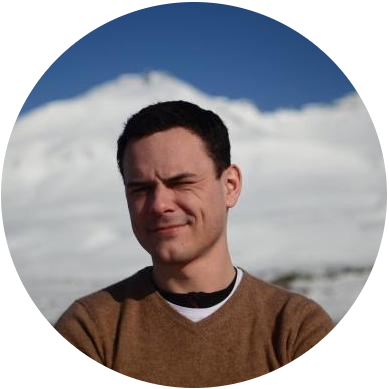
\includegraphics[width=0.6\linewidth]{./png/myphoto.png}	
\end{figure}

\begin{center}
\parbox{0.85\mpwidth}{\larrow{softcol}\textcolor{lightgray}{\textit{Traffic safety researcher with a research interest on \textbf{driver behaviour modelling} and \textbf{vulnerable road user} safety}}}
\end{center}

\begin{metasection}{Contact}

	\iconhref{map-marker-alt}{12}{Ingared, Sweden}{https://www.openstreetmap.org/?mlat=57.85313&mlon=12.46040\%23map=19/57.85313/12.46040}{white}\\[6pt]
	\icontext{mobile-alt}{12}{+46 (0)7 036 336 77}{white}\\[6pt]
	\iconemail{envelope}{12}{christian-nils.boda@gadz.org}{christian-nils.boda@gadz.org}{white}\\[6pt]
	\iconhref{globe-europe}{12}{https://christian-nils.github.io/}{https://christian-nils.github.io/}{white}\\[6pt]
	\iconhref{github}{12}{christian-nils}{https://github.com/christian-nils}{white}
	\iconhref{twitter}{12}{@christiannils}{https://twitter.com/christiannils?lang=en}{white}\\[6pt]
	\iconhref{linkedin}{12}{cboda}{https://www.linkedin.com/in/cboda/?locale=en_US}{white}\\[6pt]

\end{metasection}
	
%----------------------------------------------------------------------------------------
%	META SECTION
%----------------------------------------------------------------------------------------

\begin{metasection}{Fields}
	
	\icontext{car-crash}{12}{Traffic safety research}{white}\\[3pt]
	\icontext{user}{12}{Human factors analyses}{white}\\[3pt]
	\icontext{user-cog}{12}{Driver behaviour modelling}{white}\\[3pt]
	\icontext{biking}{12}{Vulnerable road users safety}{white}\\[6pt]
	\icontext{car-side}{12}{Automotive engineering}{white}\\[3pt]
	\icontext{cogs}{12}{Mechanical engineering}{white}\\[3pt]
	\icontext{industry}{12}{Industrial engineering}{white}\\[3pt]

\end{metasection}


\begin{metasection}{Technologies}

\textcolor{white}{
\icontext{code}{12}{MATLAB}{white}
\icontext{vuejs}{12}{Vue.js}{white}
\icontext{css3}{12}{CSS3}{white} \\[6pt]
\icontext{python}{12}{Python}{white}
\icontext{code}{12}{C/C++}{white}
\icontext{java}{12}{JAVA}{white} \\[6pt]
\icontext{js}{12}{JavaScript}{white}
\icontext{pen-fancy}{12}{LaTeX}{white}
\icontext{robot}{12}{ROS}{white}
}
\end{metasection}

\begin{metasection}{Tools}

\textcolor{white}{
\icontext{file-code}{12}{VS code}{white}\icontext{paint-brush}{12}{Inkscape}{white}\\[6pt]
\icontext{cube}{12}{Blender}{white}
}
\end{metasection}

\begin{metasection}{Activities}

\textcolor{white}{\LARGE{\icon{hiking}{24}{white} \icon{laptop-code}{24}{white}  \icon{bicycle}{24}{white}}}
\end{metasection}

\begin{metasection}{Operating Systems}

\textcolor{white}{\LARGE{\icon{linux}{24}{white} \icon{windows}{24}{white}}}

\end{metasection}


\parbox{1\mpwidth}{
	\centering
	
\includegraphics[width=0.1\linewidth]{./png/france.png}	
	\hspace{4pt}
	
\includegraphics[width=0.1\linewidth]{./png/uk.png}	
	\hspace{4pt}
	
\includegraphics[width=0.1\linewidth]{./png/sweden.png}	
}

\end{minipage}}


\fcolorbox{white}{white}{\begin{minipage}[c][0.95\textheight][t]{1\linewidth}

	%---------------------------------------------------------------------------------------
	%	EDUCATION SECTION
	%--------------------------------------------------------------------------------------
	\cvsection{Education}
	
	\cvevent{2011 - 2013}{Chalmers University of Technology, Gothenburg}{M.Sc. Automotive Engineering}{
		\begin{description}
			\item[Master thesis] in the Accident Prevention research group, Chalmers University of Technology, I developed an embedded system that automatically provided speed instruction to a professional driver to control on-road testing with participants. Several Phidgets SBC were used to setup the whole system.
		\item[Automotive Engineering Project] I took part in a project that developed a proof-of-concept Android application to provide a warning to a cyclist and a driver when their travel paths would lead to a crash. 
		\end{description}
	}
	
	\cvevent{2009 - 2011}{Arts et Métiers PARISTECH, Aix-en-Provence}{M.Sc. Industrial and Mechanical Engineering}{Ranked 92/1107, awarded with the Silver medal.}
	\cvevent{2007 - 2009}{Lycée Masséna, Nice}{Preparatory classes, MPSI-PSI, equivalent to B.Sc. Mathematics}{}
	
	\cvsection{Publications}
	\nocite{*}
	\begin{center}
	\parbox{0.95\mpwidth}{
		\setlength\bibitemsep{1.5\itemsep}
	\printbibliography[heading=none]}
	\end{center}
	\end{minipage}}%
%============================================================================%
%
%
%
%	DOCUMENT END
%
%
%
%============================================================================%
\end{document}
